%==========================================================
%--- What programs are and how they are written in our tool
%==========================================================
\section{System Model}
\label{sec:sys_model}

A data store in our system model is a collection of \emph{replicas}
(\replO{1},\replO{2},...), each of which maintains a copy of a set of
replicated \emph{data object} (\xO,\yO,...).  Each data object includes
maintains a \emph{state value} (\vO,\vO',...) and is equipped with a set of \emph{operations}
(\opO,\opO',...). Operations may read the state of an object
residing in a replica, and modify it by generating \emph{update
effects} ($\eff$,$\eff'$,...).
Update effects
or simply effects are asynchronously sent to all other replicas, where,
by using a
user-defined function, are \emph{applied} to the state of the object
instance in the recipient replica. 
Fig.~\ref{fig:sys_model1} and \ref{fig:sys_model2} illustrate this
process, where the example shows how effects are locally created and
remotely applied. 

Observe that in our system model, there is no direct synchronization between replicas when an
operation is executed, which means concurrent and possibly conflicting
updates can be generated at different replicas. We
require the user-defined \emph{apply} function to implement a conflict
resolution strategy for replicas to eventually converge. 
This model admits all inconsistencies and anomalies
associated with eventual consistency \cite{quelea,terry}, and our goal is equip
applications and implementations with mechanisms to specify and prevent
such inconsistencies. 

Clients in our model, interact with the store by invoking operations on objects.
A \emph{session} is a sequence of operations invoked by a particular
client. Consequently, operations (and effects) can be uniquely
identified by the \emph{session id} that invoked them, and
their \emph{sequence number} in that particular session, which is used
by replicas, to record the set of all updates locally applied.
Since, the data
store is concurrently accessed by a typically large number of clients,
and as a result of the load balancing regulations,
operations (even from the same session) might be routed to different
replicas (Fig.~\ref{fig:sys_model1} and
\ref{fig:sys_model3}). 


Lastly, we define two relations over effects created in the store.
\emph{Session order} ($\soZ$) is an irreflexive, transitive relation that relates
an effect to all subsequent effects from the same session.
Moreover, we define 
\emph{visibility} (${\visZ}$) 
as an irreflexive and assymetric relation that 
relates an effects to all others that are influenced by it (witnessed its
update) at the time of their generation.
For example, in Fig.~\ref{fig:sys_model3} $\visO
(\eta,\eta')$ holds, since $\eta$ (the effect of $\opO$) has already been
delivered and applied to the replica~\replO{4}, when $\opO$ is executed and thus has influenced 
generation of $\eff'$.
\begin{figure}[t]
    \centering
    \begin{subfigure}[t]{0.31\textwidth}
    \centering
        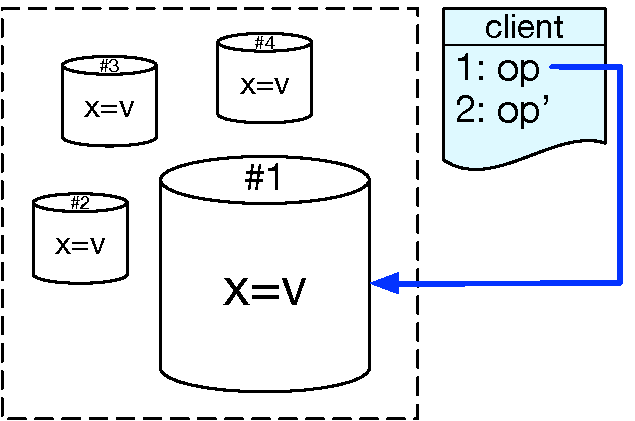
\includegraphics[scale=0.32]{Figures/system_model1.pdf}
        \caption{\scriptsize A client submits an operation op to the store, which
	is routed to the replica1.}
        \label{fig:sys_model1}
    \end{subfigure}
    \hfill
    \begin{subfigure}[t]{0.31\textwidth}
        \centering
	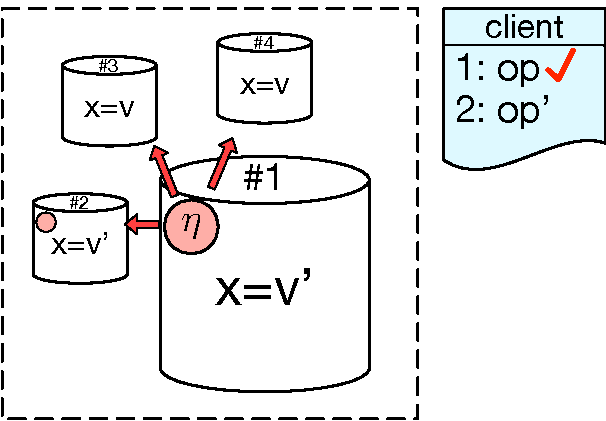
\includegraphics[scale=0.32]{Figures/system_model2.pdf}
        \caption{\scriptsize The state of the eplica1 is updated, an
	effect is created and is being propagated}
        \label{fig:sys_model2}
    \end{subfigure}
    \hfill
    \begin{subfigure}[t]{0.31\textwidth}
        \centering
	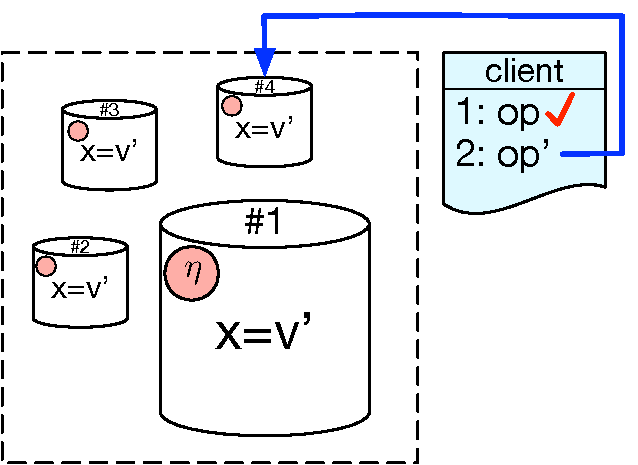
\includegraphics[scale=0.32]{Figures/system_model3.pdf}
        \caption{\scriptsize Second operation op' is submitted to the store, which
	is routed to another replica}
        \label{fig:sys_model3}
    \end{subfigure}
    \caption{system model of \tool}\label{fig:system_model}
\end{figure}




















%==========================================================




























































\begin{comment}

%
% Initial Paragraph explaining the running example
%

Let's consider the developement of a modern-day large scale \emph{Bulletin
Board} web application, that allows managers to initiate multiple boards for their
organization, where employees can either write something on the
board, or request to read all the messages on it.
In order to achieve high availablity, developers decide to implement the
application as distributed servers, working
with replicated data objects on top of an 
Eventually Consistent Data Store ({ECDS}). The data model here dictates
each row at the data base level, to include a board identifier
and a set of messages 
(Fig. \ref{fig:simple_bb}).
In this fashion, employees can start a session to send requests to geographically distributed
servers and make updates to the rows, and the underlying store,
would guarantee the eventual delivery of all updates at every server.
\begin{figure}[t]
    \begin{subfigure}[b]{0.48\textwidth}
        \centering
	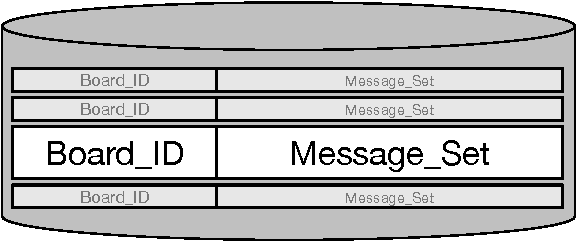
\includegraphics[scale = 0.5]{Figures/SimpleBulletinApp.pdf}
	\caption{Simple Data Model}
        \label{fig:simple_bb}
    \end{subfigure} 
    \begin{subfigure}[b]{0.48\textwidth}
        \centering
	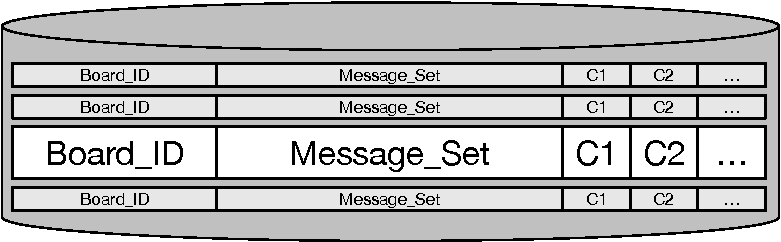
\includegraphics[scale=0.5]{Figures/ModifiedBulletinBoard.pdf}
	\caption{Modified Data Model}
	\label{fig:modified_bb}
    \end{subfigure}
    \\ \hrulefill \\
\caption{Low-Level Data Model of a Simple Bulletin Board Application
(Left) and the Modified Version Including Meta-data for Each Running
Session}
\label{fig:simple_modified_bb}
\end{figure}

%
%===========================================================================SUBSECTION
% Paragraph 2: Explaining the possible anomaly under EC
%
\subsection{Ad-hoc Anomaly Prevention Mechanisms}

Developers cannot solely rely on the eventual consistency guarantee that
is provided by the underlying data stores for application correctness. There are application integrity anomalies
that must be thought of at the developement stage and be handled. For
example, assume an employee signs into the system, writes some
messages on the board, and immediately refreshes her browser hoping to see
her messages on the board, which are however not there. This is obviously
not desirable and as mentioned in
the previous section,  can occure if
the write messages were sent to a server, and the subsequent read to
another, where her previous write updates are  not available yet. 
\begin{wrapfigure}{l}{0.3\textwidth}
	\centering
	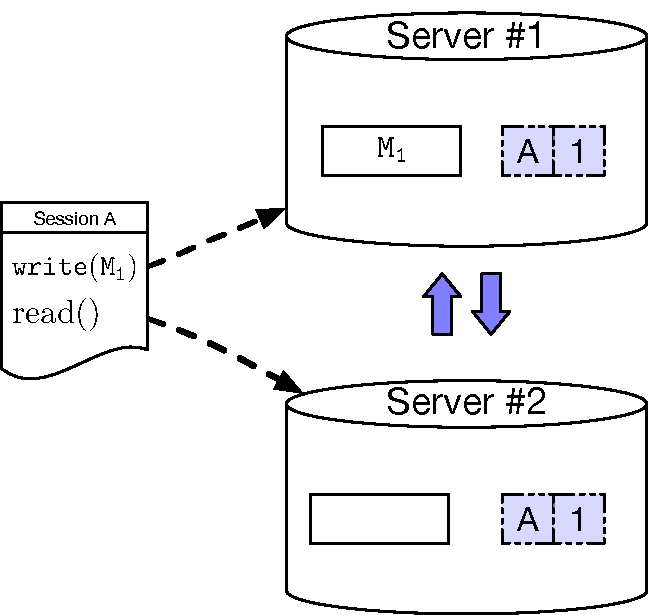
\includegraphics[scale = 0.4]{Figures/metadatapresent.pdf}
\vspace{1 mm} 
\hrule
\caption{Incorrect implementation of RMW. The meta data referring to the
first operation of session A can be present at server \#2, when the
actuall message is not}
\end{wrapfigure}

%
% Paragraph 3: Ad-hoc prevention methods
%

To prevent this anomaly, developers must provide RMW consistency
guarantee for their application, where user requests sent to a server are guaranteed to see
all the previous updates made by the same client and session. The
conventional technique for acheiving this,
is to tag each session and its contained requests, respectively with unique identifiers and
sequence numbers and to include this meta-data in the database, to
record what requests have been seen by the server at any time. 
Moreover, there must be some mechanisms to temporarily block user requests, when the database
does not include the updates from previous requests.
Since developers are not interested in synchronized and direct
communication between servers (which obviously contradics the idea of using
an ECDS), they have to record the meta data in the key value store and rely on
the provided delivery mechanisms. 
%
%Paragraph 4: The problem with simply adding the metadata on top of the
%implementation
%

However, the desired behavior cannot
be achieved by simply creating meta data "add-ons" to the current implementation.
The reason is that, in EC stores, no order of delivery is guaranteed,
and some servers might receive the meta-data regarding some updates that
are not present at the server yet. 
Developers need to make sure that the meta-data recording sequence
number of a request, becomes available at a server, at the same time
when the corresponding update arrives. This can only be done by
modifying the low-level initial data models, to also record the sequence
numbers seen from each client. 
%
% Paragraph 5: The difficulties of low-level modifications: complex
% and redundant
%

Now developers are inevitebaly required to modify the origianl low level
data model to also include the required meta data, so the changes in the
data and meta-data would arrive at servers atomically. Such changes on
the data model will require rewriting 90\% of application functions from the scratch
which is extremely inconvinience. 
Moreover, now developers must face non-trivial problems associated with
session management and dynamic data models. For example, when a new
client arrives at a server 
and initiates a session, the server is required to generate a unique ID
for that session, and then add a new column to the
underlying database table, to record the associated meta-data.
Unfortunately, table alteration in ECDSs is not an atomic task, and forces developers to implement
appropriate guards to make sure that the new column is available at all servers, before
allowing the client to move on with the rest of her requests.  
%
% Paragraph 6: The problem of new consistency requirements
%

To make the matter worse, new integrity anomalies are discovered very
frequently. Assume the bulltin board application with RMW has been
successfully designed and implemented, however, after the developement
phase users report a new type of anomaly, where messages seem to be
disappeared after refreshing the browser. This undesirable behavior is
allowed under EC and even RMW; since two read operations can go to
different servers, where the second one does not include all the
messages read from the first server. This requires another consistency
level, called Monotonic Reads, that guarantees subsequent reads will
include everything that has been read before in a session.
 
 
 






\end{comment}


